
\chapter{Software Architektur}
\section{Anforderungen}
\label{sec:Anforderungen} 
%Christoph

Im Folgenden sollen die Anforderungen an die Studienarbeit festgelegt werden. Diese gliedern sich in vier Hauptbestandteile auf. \newline
Der \textbf{erste Teil} besteht darin, ein bestehendes Vorgängerprojekt in eine andere Umgebung zu portieren. Das Projekt ermöglicht die Steuerung einer AR.Drone 2.0 mit Hilfe von Gesten. Die Gesten sind vorgeschriebene Positionen der Arme. So soll der Nutzer beispielsweise mit einer Bewegung von beiden ausgestreckten Armen, nach oben und unten, die Drohne starten, steigen, senken und landen lassen können. \newline
Dabei wurde die Erkennung der Positionen mit eines Kinect Sensors von Microsoft umgesetzt. Die Bilddaten der Kamera werden im Programmcode verarbeitet und mit Fuzzylogik analysiert. Dieser wurde in der Programmiersprache \textit{C\#} geschrieben und funktioniert auf Grund einer Vielzahl von externen Bibliotheken, wie die Anbindung der Kinect, nur unter dem Betriebssystem Microsoft Windows. \newline 
Als Grundlage für die weiteren Ziele dieser Arbeit soll dieses Projekt für UNIX basierte Betriebssysteme umgeschrieben werden. Grundlage für die Softwarearchitektur bildet das ROS Framework, welches eine Modularisierung der Projektbestandteile in ROS Nodes vorgibt. Ziel soll es sein, die Funktionalität des Bestandsprojektes vollständig nachzubilden. \newline
Der \textbf{zweite Anforderungsteil} besteht darin, dass jegliche Funktionalität auch in einer Simulation verfügbar sein soll. Somit kann man in Situationen, in denen der Flug einer Drohne nicht möglich ist, den Quadrocopter in einer frei gestaltbaren, simulierten Umgebung fliegen lassen. Weiterhin ist es dadurch möglich Funktionalitäten sicherer und ohne Risiko zu testen.
Es soll in diesem Zusammenhang möglich sein, problemlos zwischen einer realen und einer simulierten Drohne wechseln zu können.\newline
Ein \textbf{weiterer Bestandteil} dieser Arbeit umfasst die Approximation von Tiefeninformationen. Dafür soll ausschließlich eine unveränderte AR.Drone verwendet werden, welche nur mit einer monokularen Frontkamera ausgestattet ist. \newline
Um aus den Bildern dieser Kamera Tiefenbilder zu gewinnen, soll ein externes Projekt in die Projektlandschaft integriert werden. Hierbei soll es wiederum möglich sein, dass der Videostream sowohl von der realen, als auch von der simulierten Drohne gesendet werden kann. Es soll dabei ermittelt werden, ob die Nutzung der externen Arbeiten für den Anwendungszweck praktikabel und sinnvoll ist. \newline
Der \textbf{vierte Bestandteil} dieser Arbeit besteht im Erarbeiten, Testen, Bewerten von möglichen Ansätzen und Limitationen der Implementierung eines Assistenzsystems. Das Ziel ist es herauszufinden, wie mit den Tiefeninformationen die manuelle Steuerung der Drohne durch eine Person, mit Hilfe von Assistenzfunktionen, unterstützt werden kann. \newline
Ein Anwendungsbeispiel ist hierbei das sichere Fliegen durch ein Hindernis wie eine offene Tür, oder das Verhindern von Kollisionen mit Objekten in der Umgebung.
\newpage
\section{Bildverarbeitung}
\label{Bildverarbeitung}
In diesem Abschnitt wird beschrieben, wie die Position der Kamera im Raum bestimmt werden kann, um anschließend aus aufeinanderfolgenden Aufnahmen Tiefeninformationen zu gewinnen. Die beschriebenen Implementierungen beziehen sich dabei auf die Arbeit von Christian Forster, et al. \cite{Forster2014ICRA}, welche ihre Abhandlungen zum Thema zusammen mit dem Programmcode frei zugänglich gemacht haben.

\subsection{Semi-Direct Monocular Visual Odometry - SVO}
%Christoph
Eine Grundanforderung an das Projekt ist die Nutzung einer nicht modifizierten AR.Drone. Dadurch entsteht die Problematik, dass keine Tiefenbildkamera genutzt werden kann, um in Echtzeit Tiefenbilder zu erhalten. Die Drohne ist lediglich mit einer monokularen Frontkamera ausgestattet. \newline
Um Tiefeninformationen aus den Bildern einer solchen Kamera zu gewinnen, wird eine Szene aus verschiedenen Perspektiven aufgenommen. Anschließend gibt es unterschiedliche Ansätze um aus den aufeinanderfolgenden Bildern Kamerapositionen und Umgebungsstrukturen zu ermitteln. \newline
Feature basierte Ansätze sind der aktuelle Standard zur Berechnung der Kameraposition. Diese versuchen die wichtigsten Merkmale eines Bildes, die Features, zu extrahieren. Mit Hilfe von Feature Deskriptor Algorithmen werden Vektoren mit Informationen zu invarianten Bildbereichen berechnet. Diese Vektoren verhalten sich wie ein einzigartiger Fingerabdruck, der die Merkmale repräsentiert. \newline
Aufeinanderfolgende Bilder werden dann mit Hilfe dieser Deskriptoren abgeglichen und sowohl Kamerabewegungen, als auch Strukturen werden rekonstruiert. Zur Optimierung sind abschließend die ermittelten Kamerapositionen anzugleichen. Dies geschieht mit Hilfe von Algorithmen zur Minimierung des Reprojektionsfehlers.\footnote{Reprojektionsfehler sind geometrische Fehler die im Zusammenhang zwischen abgebildeten und berechneten Bildpunkten entstehen. \cite{repro}} 
\newline
Ein weiterer Ansatz ist die direkte Methode. Hierbei werden die Features nicht über Deskriptor Algorithmen bestimmt, sondern das Problem wird über die Intensitäten der Pixel gelöst. Bei einem Graustufenbild entspricht diese Intensität der Helligkeit von Bildbereichen.
Somit kann bei der Rekonstruktion im Gegensatz zum Feature basierten Ansatz auch die Richtung der Gradienten von Intensitäten genutzt werden. Dadurch funktioniert diese Methode auch bei Bildern mit sehr wenig Textur, Bewegungsunschärfe und fehlerhaftem Kamerafokus. \newline
Das für diese Arbeit relevante Vorgehen kombiniert die Vorteile der beschriebenen Methoden. Die semi-direkte Odometrie\footnote{Odometrie bezeichnet die Verwendung Bewegungssensordaten zur Bestimmung der Positionsänderung über die Zeit.\cite{hodor}} verwendet einen Algorithmus der ebenfalls auf Zusammenhängen von Features basiert. Diese werden jedoch implizit aus einer direkten Bewegungsabschätzung bezogen, anstatt explizit durch Algorithmen mit Feature Deskriptoren berechnet zu werden. 
Dadurch müssen Features nur extrahiert werden, wenn diese noch nicht auf einem der vorherigen Bildern vorhanden waren. \newline
Insgesamt ist dieser Ansatz sehr performant, da wenig Berechnungen pro Bild stattfinden und ist aufgrund der Verwendung von Intensitätsgradienten äußerst genau und robust. \newline
Diese Eigenschaften sind für die Anforderungen dieser Arbeit essentiell, da die Drohne sich sehr schnell bewegen kann und somit in möglichst kurzer Zeit neue Bilder auswerten muss. Das beschrieben Verfahren minimiert damit die Auswirkungen der typischen Probleme von Drohnen. Diese sind einerseits die niedrige Texturierung der Umgebung, welche hauptsächlich in Innenräumen auftritt und andererseits kameraspezifische Probleme wie Bewegungsunschärfe und der Verlust des Kamerafokus. \newline
Im Folgenden zeigt die Abbildung wie die Nutzung von SVO in der Praxis aussieht.
\begin{figure}[ht]
	\centering
	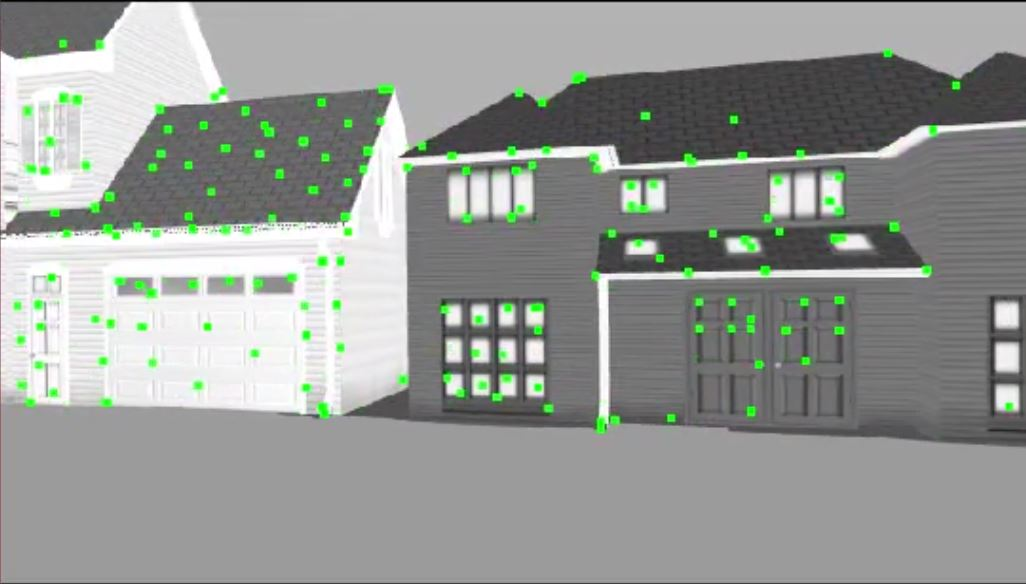
\includegraphics[scale=0.7]{Bilder/SVO.jpg}
	\label{fig:svo}
	\caption{Semi-Direct Monocular Visual Odometry im Simulator}
\end{figure}

Hierbei stammt das Kamerabild von einer Drohne im Simulator Gazebo in einer frei verfügbaren Testwelt mit einigen Gebäuden. Die grünen Punkte sind die Features, die SVO anhand der beschriebenen Strategie ermittelt hat. \newline
Die Anzahl der aktuell gefundenen Features kann dabei stark variieren. Diese Schwankung entsteht hauptsächlich durch die unterschiedliche Texturierung und Anzahl der Kanten von Objekte in der Umgebung. \newline
Weiterhin kann auch die Kamera selbst ein Grund für eine geringe Anzahl gefundener Features sein. Gründe und Lösungen dafür werden im Folgenden beschrieben.

\subsection{Kamerakalibrierung}
%Christoph
Ein Grundproblem der Bildverarbeitung ist die Verzerrung des Bildes. 
Da die Bestimmung der Kameraposition möglichst genau sein soll, muss die Kamera vorher kalibriert werden. Dies bedeutet, dass Ungenauigkeiten der Linse erkannt und von Seiten der Software ausgeglichen werden. Dafür werden die intrinsischen Parameter der Kamera bestimmt. \newline
\subsubsection*{Kalibrierungsmodelle}
Hierbei unterstützt SVO drei Kamera Modelle: ATAN, Ocam und Lochkamera. \cite{svo_cameracalibration} \newline
Das ATAN Modell basiert auf dem \textit{Field of View \emph{(FOV)}} Verzerrungsmodell \grqq Straight lines have to be straight [...]\grqq von Devernay und Faugeras. \cite{calibration}\newline %cite https://hal.inria.fr/inria-00267247/document
Der Vorteil dieser Kalibrierungsmethode ist die äußerst schnelle Berechnung der Projektion des Bildes.\cite{calibration2} % cite https://github.com/uzh-rpg/rpg_svo/wiki/Camera-Calibration
Das Modell vernachlässigt jedoch tangentiale Verzeichnung, welche auftritt, wenn optische und mechanische Bestandteile des Objektives, sowie der CCD-Sensor 
\footnote{CCD steht für \emph{charge-coupled device}, was übersetzt ladungsgekoppeltes Bauteil bedeutet. Dieses lichtempfindliche elektronische Bauteil wird zur Bildaufnahme verwendet.} 
nicht perfekt zueinander ausgerichtet sind.\cite{calibration3} % cite http://www.aishack.in/tutorials/major-physical-defects-cameras/
Weiterhin sollte die Kamera mit einem globalem Shutter ausgestattet sein, um die Extraktion von Bildmerkmalen bei Bewegungen zu gewährleisten. Kameras mit Global-Shutter-CMOS  
\footnote{CMOS steht für \emph{Complementary metal-oxide-semiconductor} und ist ein spezieller Halbleiter der zur Bildaufnahme verwendet wird.\cite{CMOS}} % cite https://de.wikipedia.org/wiki/Complementary_metal-oxide-semiconductor
Sensoren und CCD-Sensoren nehmen Bild nicht zeilen- und spaltenweise, sondern vollständig auf und sind daher für das Verfahren geeignet. \newline
Die Drohne besitzt eine veraltete und günstige Kamera mit einem CMOS Sensor, wodurch sowohl tangentiale Verzerrung, als auch der Rolling-Shutter-Effekt auftreten können.\cite{developerGuide} \newline
%cite https://dspace.cvut.cz/bitstream/handle/10467/66885/F3-DP-2017-Pahorecky-Petr-priloha-ARDrone_Developer_Guide.pdf?sequence=-1&isAllowed=y
Daher ist das ATAN Modell zwar eine der besten Kalibrierungsmethoden für teure Hochleistungskameras, jedoch ist es für die Betrachtungen dieser Arbeit nicht optimal. \newline 
Der zweite Ansatz zur Kalibrierung ist das Ocam Modell von Davide Scaramuzza \cite{scaramuzza}. Diese Methode sollte für Kameras mit sehr weitem Sichtfeld, oder omnidirektionalen Kameras genutzt werden. Damit ist es für die Drohne nicht geeignet. \newline
Die dritte unterstützte Kalibrierungsmethode ist das Modell der \textit{Lochkamera}, bzw. auf Englisch \textit{Pinhole Model}.
Der Name und das zugrunde liegende Prinzip basieren, wie der Name es sagt, auf der Lochkamera. Die Abbildung zeigt die grundsätzliche Funktionsweise. \newline
\begin{figure}[ht]
	\centering
	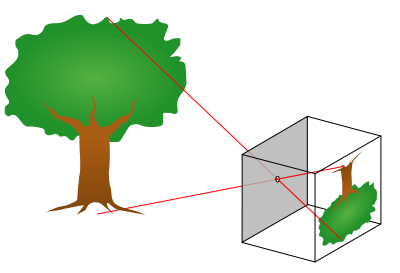
\includegraphics[scale=0.5]{Bilder/pinhole.png}
	\label{fig:pinhole}
	\caption{Prinzip der Lochkamera \cite{lochkamera}}
\end{figure}

Die Darstellung zeigt, dass bei der Lochkamera Licht durch eine kleine Öffnung in einen kleinen Hohlkörper fällt. Dadurch entsteht auf der Rückseite ein auf dem Kopf stehendes Bild. \newline
Bei dem Pinhole Model handelt es sich um den aktuellen Standard in OpenCV \footnote{``OpenCV is the leading open source library for computer vision, image processing and machine learning, and now features GPU acceleration for real-time operation.''\cite{opencv}} %cite https://developer.nvidia.com/opencv
und ROS. Hierbei wird die Verzerrung mit Hilfe von fünf intrinsischen Parametern beschrieben, welche im Rahmen der Kalibrierung bestimmt werden müssen.

\begin{figure}[ht]
	\centering
	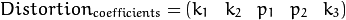
\includegraphics[scale=0.7]{Bilder/distortion.png}
	\label{fig:distortion}
\end{figure}

OpenCV betrachtet dabei radiale und tangentiale Faktoren. Die Formel für radiale Verzeichnung ist die Folgende:

\begin{figure}[ht]
	\centering
	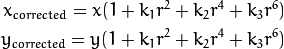
\includegraphics[scale=0.7]{Bilder/radialFactors.png}
	\label{fig:radial}
\end{figure}

Hierbei wird aus einem alten Bildpunkt $(x,y)$ des Eingabebildes die korrigierte Position $x_{corrected} y_{corrected}$ bestimmt. \newline
Die Berechnung der tangentialen Verzerrung erfolgt durch die Formel:

\begin{figure}[ht]
	\centering
	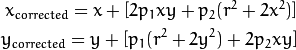
\includegraphics[scale=0.7]{Bilder/tangentialFactors.png}
	\label{fig:radial}
\end{figure}

Abschließend werden die Einheiten angepasst:

\begin{figure}[ht]
	\centering
	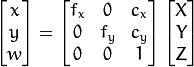
\includegraphics[scale=0.7]{Bilder/matrixEquation.png}
	\label{fig:radial}
\end{figure}

Dabei entspricht $f_x$ und $f_y$ der Brennweite der Linse und $c_x$, sowie $c_y$ beschreiben die optische Bildmitte in Pixelkoordinaten. \cite{cameracalibration}\newline
% cite http://docs.opencv.org/2.4/doc/tutorials/calib3d/camera_calibration/camera_calibration.html
Dieser Ansatz ist der einfachste und funktioniert grundsätzlich mit jeder Kamera.

\subsubsection*{Umsetzung der Kalibrierung}
Um die intrinsischen Parameter der Kamera zu bestimmen, wird ein bekanntes Bild oder Muster aufgenommen. Dazu wird ein Vergleich zwischen den theoretischen und tatsächlichen Abmessungen angestellt. Hierzu wird meist ein einfaches Schachbrettmuster genutzt, welches im möglichst vielen verschiedenen Perspektiven aufgenommen wird. Bei der realen Drohne wird dazu das Muster ausgedruckt, bei der Simulation muss hingegen ein muss ein solches Objekt in die Welt eingefügt werden. Da die Kamera in der Simulation ohnehin keine intrinsischen Fehler aufweisen sollte, kann auf eine Kalibrierung verzichtet werden. \newline

\begin{figure}[ht]
	\centering
	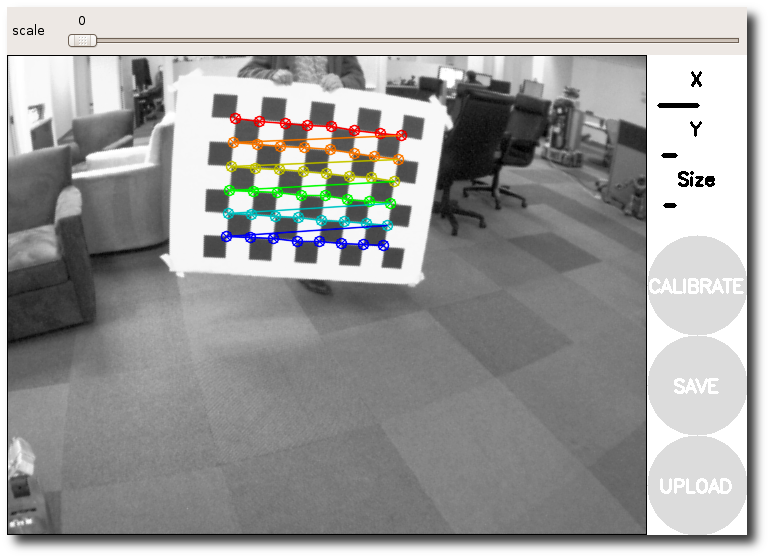
\includegraphics[scale=0.4]{Bilder/calibrationChecker.png}
	\label{fig:calibrationChecker}
\end{figure}
%todo: Quelle + Titel
Die Kalibrierung wurde mit dem frei verfügbaren ROS Node \textit{camera\_calibration} umgesetzt. Das Ergebnis ist abhängig von der Anzahl der Perspektiven und der Qualität der Aufnahmen. Aufgegeben wird dann die List der Parameter, die für das Lochkamera Modell notwendig sind.

\subsection{Regularized Monocular Depth Estimation - REMODE}
%Christoph
Im vorherigen Abschnitt wurde beschrieben, wie anhand von aufeinanderfolgenden Bildern die Position der Kamera im Raum bestimmt werden kann. Dieses Problem wird seit mehr als 20 Jahren untersucht und wird als Structure From Motion \emph{SFM} in der Bildverarbeitung und Simultaneous Localization and Mapping \emph{SLAM} in der Robotik bezeichnet. \newline
%Smith, R.C.; Cheeseman, P. (1986). "On the Representation and Estimation of Spatial Uncertainty" (PDF). The International Journal of Robotics Research. 5 (4): 56–68. 
Um den Nutzer aktiv bei der Steuerung der Drohne zu unterstützen werden jedoch Tiefeninformationen benötigt. Dazu müssen Tiefenbilder und Tiefenkarten (footnote) aus den Bildern der monokularen Kamera bestimmt werden. \newline
Für diesen Schritt gibt es unterschiedliche Ansätze. Der State of the Art ist die Berechnung mit Hilfe des Bayes-Schätzers. Dabei handelt es sich um eine Schätzfunktion in der mathematischen Statistik, welche eventuell vorhandenes Vorwissen bei der Schätzung eines Parameters berücksichtigt. Dabei wird in der bayesschen Statistik das initiale Vorwissen mit Hilfe der A-priori-Verteilung modelliert, die bedingte Wahrscheinlichkeit des Parameters unter Betrachtung dieses Vorwissens mit der A-posteriori-Verteilung. \newline
%http://www.mathematik.uni-ulm.de/stochastik/lehre/ss04/statistik1/skript/node26.html
Im Umfang dieser Arbeit wird die Forschung und Implementierung des Projekts Regularized Monocular Depth Estimation \emph{REMODE} genutzt. In dieser Ausarbeitung von Matia Pizzoli, et al. \cite{Forster2014ICRA} wird die bayessche Schätzung mit neusten Entwicklungen in der Konvexoptimierung verbunden. Hierbei stützen sie ihre Forschungen auf die Ergebnisse von G. Vogiatzis und C. Hernandez und ihrer Abhandlung mit dem Titel ''Video-based, real-time multi-view stereo`` von 2011. \newline
REMODE ermöglicht mit Hilfe der gewonnenen Informationen ein dreidimensionales Modell des Raumes zu erstellen. Die Abbildung zeigt ein mögliches Anwendungsbeispiel wo Tiefeninformationen über einem Trümmerfeld gesammelt werden. \newline

\begin{figure}[ht]
	\centering
	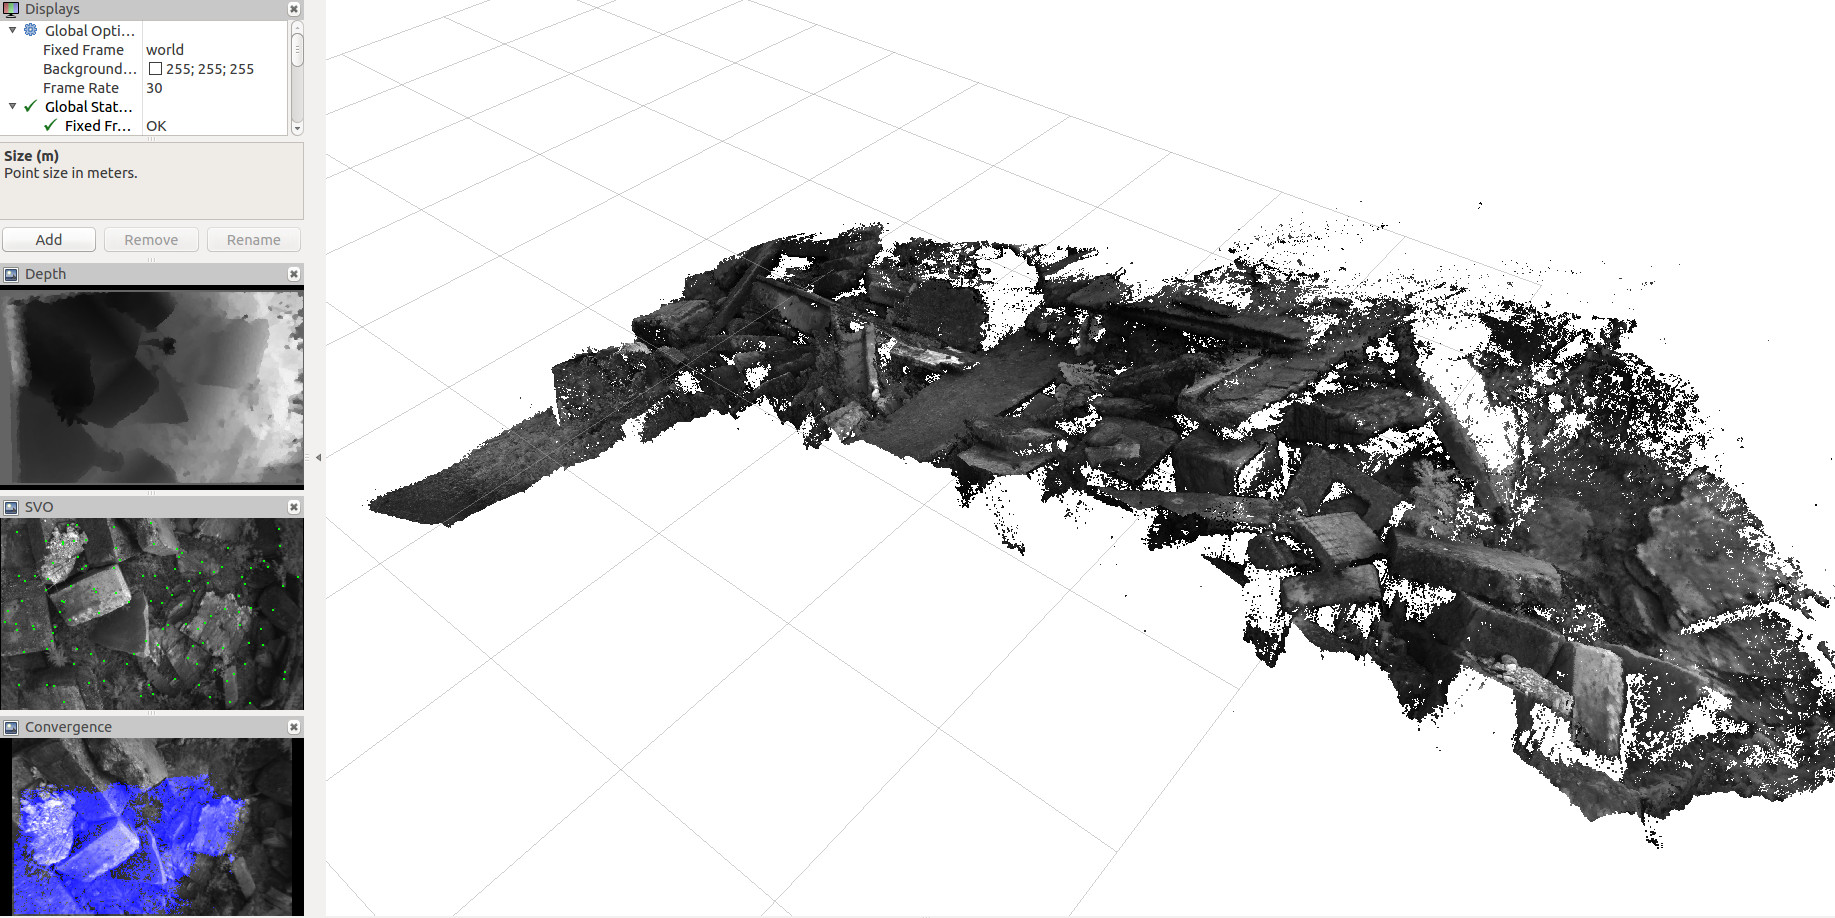
\includegraphics[scale=0.22]{Bilder/remode_3dmodel.jpg}
	\label{fig:pinhole}
	\caption{REMODE 3D-Modell, Flug über Trümmer \cite{remode3d}}
\end{figure}

Die Darstellung zeigt ein 3D Modell eines Trümmerhaufens, welches mit Hilfe der aufeinanderfolgenden Einzelbildern generiert wurde. Die Visualisierung erfolgte mit dem Standard 3D Visualisierungstool für ROS, genannt \textit{RVIZ}. \newline
REMODE ermöglicht eine Berechnung der Tiefeninformationen in Echtzeit und auf Pixelbasis. Weiterhin ist die aktuelle Genauigkeit und Fehlerrate im Vergleich zur Realität zu jeder Zeit sichtbar. \newline
Im Folgenden wird der grundsätzliche Ansatz der Implementierung skizziert. Die genauen Details übersteigen dabei auf Grund der hohen Komplexität den Umfang dieser Arbeit.

\begin{figure}[ht]
	\centering
	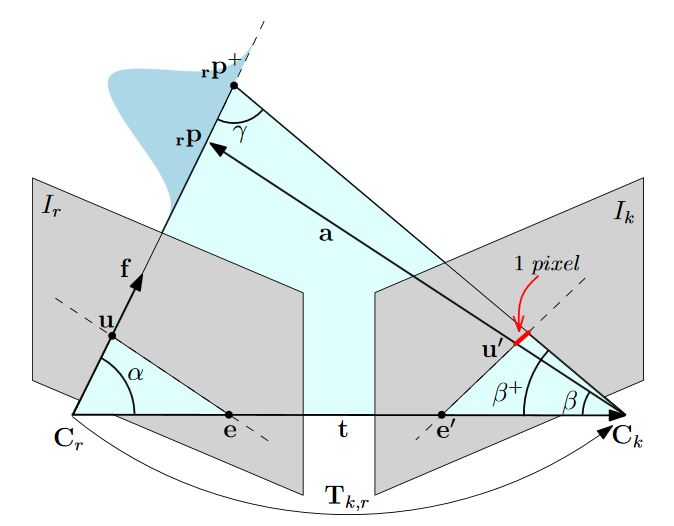
\includegraphics[scale=0.7]{Bilder/REMODE_overview.jpg}
	\label{fig:radial}
\end{figure}
%todo: Quelle + Titel
In der Übersicht sieht man die beiden Kamerapositionen $I_r$ und $I_k$ mit den zugehörigen Kamerazentren $C_r$ und $C_k$. Die Positionen im Raum dieser Kameras wurden im vorherigen Schritt mit Hilfe von SVO ermittelt. $T_k,r$ zeigt dabei die starre Transformation der Kamerabilder. \newline
Der Punkt $r_P$ ist die aktuelle Schätzung der Position eines Punktes auf den epipolaren Flächen.
Die Varianz der Abweichung von einem Pixel auf der epipolaren Linie durch estrich und ustrich wird berechnet mit der Gleichung tkquadr.
Mit Hilfe der oben angesprochenen mathematischen und statistischen Auswertungen kann nun die Tiefe eines Punktes $r_P$ approximiert werden. \newline %todo : estrich und ustrich anpassen
Das Zusammenspiel von SVO und REMODE ist für handelsüblichen Laptops mit CPU und GPU ausgelegt. Dabei führt SVO seine Berechnungen komplett auf der CPU, während REMODE die Berechnungen mithilfe des Frameworks NVIDIA CUDA \footnote{text zu CUDA} auf die Grafikeinheit des Rechners auslagert. \newline
Die Implementation setzt auf eine durchschnittliche Bewegung der Kamera von 0.0038 Meter pro Sekunde und einer mittleren Tiefe von einem Meter bei einer Berechnungszeit von 3.3 ms pro Bild. \newline
%todo referenz, footnote


\subsection{Performanceprobleme}
\label{performanceprobleme}
%hier mal vollkommen auslassen über alle performanceissues

Trotz der Nutzung neuster Methoden und Techniken zur Berechnung der Kamerapositionen und Tiefenbilder, gibt es Probleme hinsichtlich der Performance. Dabei ist das Hauptproblem die Differenz im verfolgten Ziel zwischen dieser Arbeit und der Implementierung von SVO und REMODE. \newline
Der Hauptanwendungszweck ist ein langsamer, stetiger Flug einer Drohne über ein Gebiet. Dabei zeigt die aufnehmende Kamera nach unten und hat sowohl eine sehr hohe Qualität, als auch ein großes Sichtfeld von mehr als 110 Grad. Die Bewegungen der Drohne sind nur nach seitlich, nach vorne und nach hinten, nicht jedoch um die eigene Achse. Somit wird sicher gestellt, dass immer genügend Referenzfeatures vorhanden sind, damit zu jedem Zeitpunkt die Position der Kamera bekannt ist. \newline
Im Gegensatz dazu sind die Anforderungen der Arbeit stark abweichend. So ist sowohl die Qualität, als auch die Verarbeitung der Kamera minderwertig. Auch das Blickfeld ist mit 90 Grad deutlich zu klein, wodurch weniger Features auf einem Bild Platz finden. \newline
Dadurch, dass die Kamera nach vorne und nicht nach unten gerichtet ist, treten weitere Komplikationen auf. Gleiche Bewegungen verursachen somit größere Änderungen am Bild, wodurch mehr Berechnungen notwendig werden und somit die Fehleranfälligkeit steigt. Vor allem Drehbewegungen um die eigene Achse sorgen für erhebliche Änderungen und führen meist dazu, dass SVO die aktuellen Features verliert und die Berechnungen gestoppt werden. \newline
Auch die Kalibrierung der Kamera der realen Drohne war auf Grund der schlechten Qualität schwierig. So konnte der Richtwert des Reprojektionsfehlers von rund 0,1 Pixel nicht erreicht werden, sondern lag bei 0,3 Pixel. \newline
Bei Tests in Innenräumen mit der AR.Drone konnte SVO nicht mehr als 50 Features finden. Um jedoch die Position der Kamera zu bestimmten, sind mehr als 100 Features notwendig.
Diese Beobachtungen aus den Testläufen decken sich mit den Hinweisen zur Performance in der Projektdokumentation von SVO\cite{svodocs}. \newline


\newpage
\section{Implementierung}
\subsection{Grundlegende Herausforderungen}
Als Grundlage diente eine nicht modularisierte, schlecht dokumentierte C\# Implementierung für das Betriebssystem Microsoft Windows. Diese galt es teilweise für ROS zu übernehmen. Für Windows existiert ein Kinect Software Development Kit, welches die Programmierung erleichtert. Ein weiteres generelles Problem war die Versionsinkompatibilitäten verschiedener ROS-Nodes untereinander, der ROS-Version oder mit der Betriebssystemversion. Hierbei ist es notwendig das Zusammenspiel verschiedenster Versionen zu testen und zwischen Alternativen abzuwägen. 

%\newpage
\subsection{Architektur}
%Max
Die Architektur der Anwendung wird maßgeblich durch die Verwendung des Robotic Operating System geprägt, da es eine rahmenartige Struktur bildet. Durch dieses frameworkartige Verhalten bestimmt es vorrangig die Programmstruktur, welche hauptsächlich aus verschiedenen Nodes besteht. Grob betrachtet kann man sie in zwei grundlegende Bereiche trennen:
\begin{itemize}
	\item Assistenzsystem
	\item Steuerung des Quadrocopters
\end{itemize}
Die Bereiche sind isoliert voneinander nicht nutzbar, zwar können sie ihren Zweck gut erfüllen, allerdings werden die Ergebnisse nicht verwertet. Dadurch ist die Kommunikation der Bestandteile für ein optimal funktionierende Anwendung essentiell. \newline
Ein wesentlicher Anforderung an die Architektur ist, das Simulator und Drohne ohne großen Aufwand ausgetauscht werden können. Hier hilft wiederum die ROS Umgebung dies optimal zu realisieren, da durch die lose gekoppelten Nodes, die lediglich mit Hilfe eines Message Brokers kommunizieren, Komponenten einfach ausgetauscht werden können. Ob das Projekt mit oder ohne Simulator gestartet ist über die Wahl einer entsprechenden Konfigurationsdatei, auch bezeichnet als Launch File, wo je nach dem entweder der Treiber für den realen Quadrocopter oder lediglich die Simulationsumgebung gestartet wird. Ebenfalls austauschbar ist die Art der \textbf{Steuerung des Quadrocopters}. Zwar liegt die Kontrolle via Kinect im Fokus, dennoch ist es möglich einen zusätzlichen Tastaturkontroller zu starten und diesen sogar parallel zu betreiben, da die Ansteuerung über ein und dieselbe Topic geschieht. Dies bietet auch Freiraum für zusätzliche Erweiterungen um zur Steuerung mit Kinect noch einen Spotter einzubringen, der im Notfall eingreifen kann.\newline %todo Spotter eklären
Die Steuerung durch Gesten wird im Kinect Controller realisiert, in dem die Bilddaten des optischen Sensors eingelesen werden. Zunächst wird der Nutzer erkannt, anschließend dessen Bewegungen getrackt und anhand dessen mit Hilfe von Fuzzy Logik ein Steuerbefehl erzeugt. Auf die konkrete Implementierung wird in den nachfolgenden Abschritten näher eingegangen.\newline
Die Hauptaufgabe des \textbf{Assistenzsystem} ist die Verarbeitung der Bildeingaben und einer eventuellen Korrektur der Steuerbefehle zum Vorteil des Benutzers.
Die Bilddaten des Quadrocopters, sowie auch die Bilder des Simulators werden über dieselbe Topic versandt, wodurch es wiederum keinen Unterschied für die Bildverarbeitung macht, ob die Daten simuliert sind oder es sich um ein reales Geschehen handelt. Diese Kameraaufnahmen werden Frame für Frame an die SVO-Node gesendet, wo anhand der Bildverschiebung, welche durch eine leichten Driftbewegung des Quadrocopters bedingt wird, Features berechnet und anschließend getrackt werden. Diese Featuredaten können von der REMODE-Node nachfolgend verarbeitet werden und mit deren Hilfe wird versucht ein Tiefenbild beziehungsweise eine Punktwolke zu erstellen. Die Punktwolke kann anschließend analysiert werden, wobei hauptsächlich versucht wird Hindernisse und Öffnungen, zum Beispiel Türen oder Fenster, zu erkennen und je nach aktuellem Befehlsstatus eventuell einzugreifen und dem Nutzer zu assistieren. Für bestimmte Konstellation können vorgefertigte Steuerungsabläufe durchgeführt werden um den Quadrocopter zum Beispiel durch ein Fenster zu führen oder um zu verhindern, dass er gegen eine Wand oder Hindernis fliegt. \newline
Ebenso ist theoretisch das Assistenzsystem komplett austauschbar oder durch ein Zusätzliches erweiterbar. Das ist möglich, da die Befehle in der Steuereinheit vom Kinect Controller priorisiert werden. Sofern dies intelligent geschieht, lässt sich das System um eine Vielzahl von Assistenten erweitern. Die Abbildung \ref{fig:architecture} stellt eine grob vereinfachte Visualisierung der Architektur dar und dient dazu, einen groben Überblick zu schaffen wie die Komponenten miteinander in Relation stehen. Im Folgenden werden die konkret implementierten Bestandteile genauer betrachtet.

\begin{figure}[ht]
	\centering
	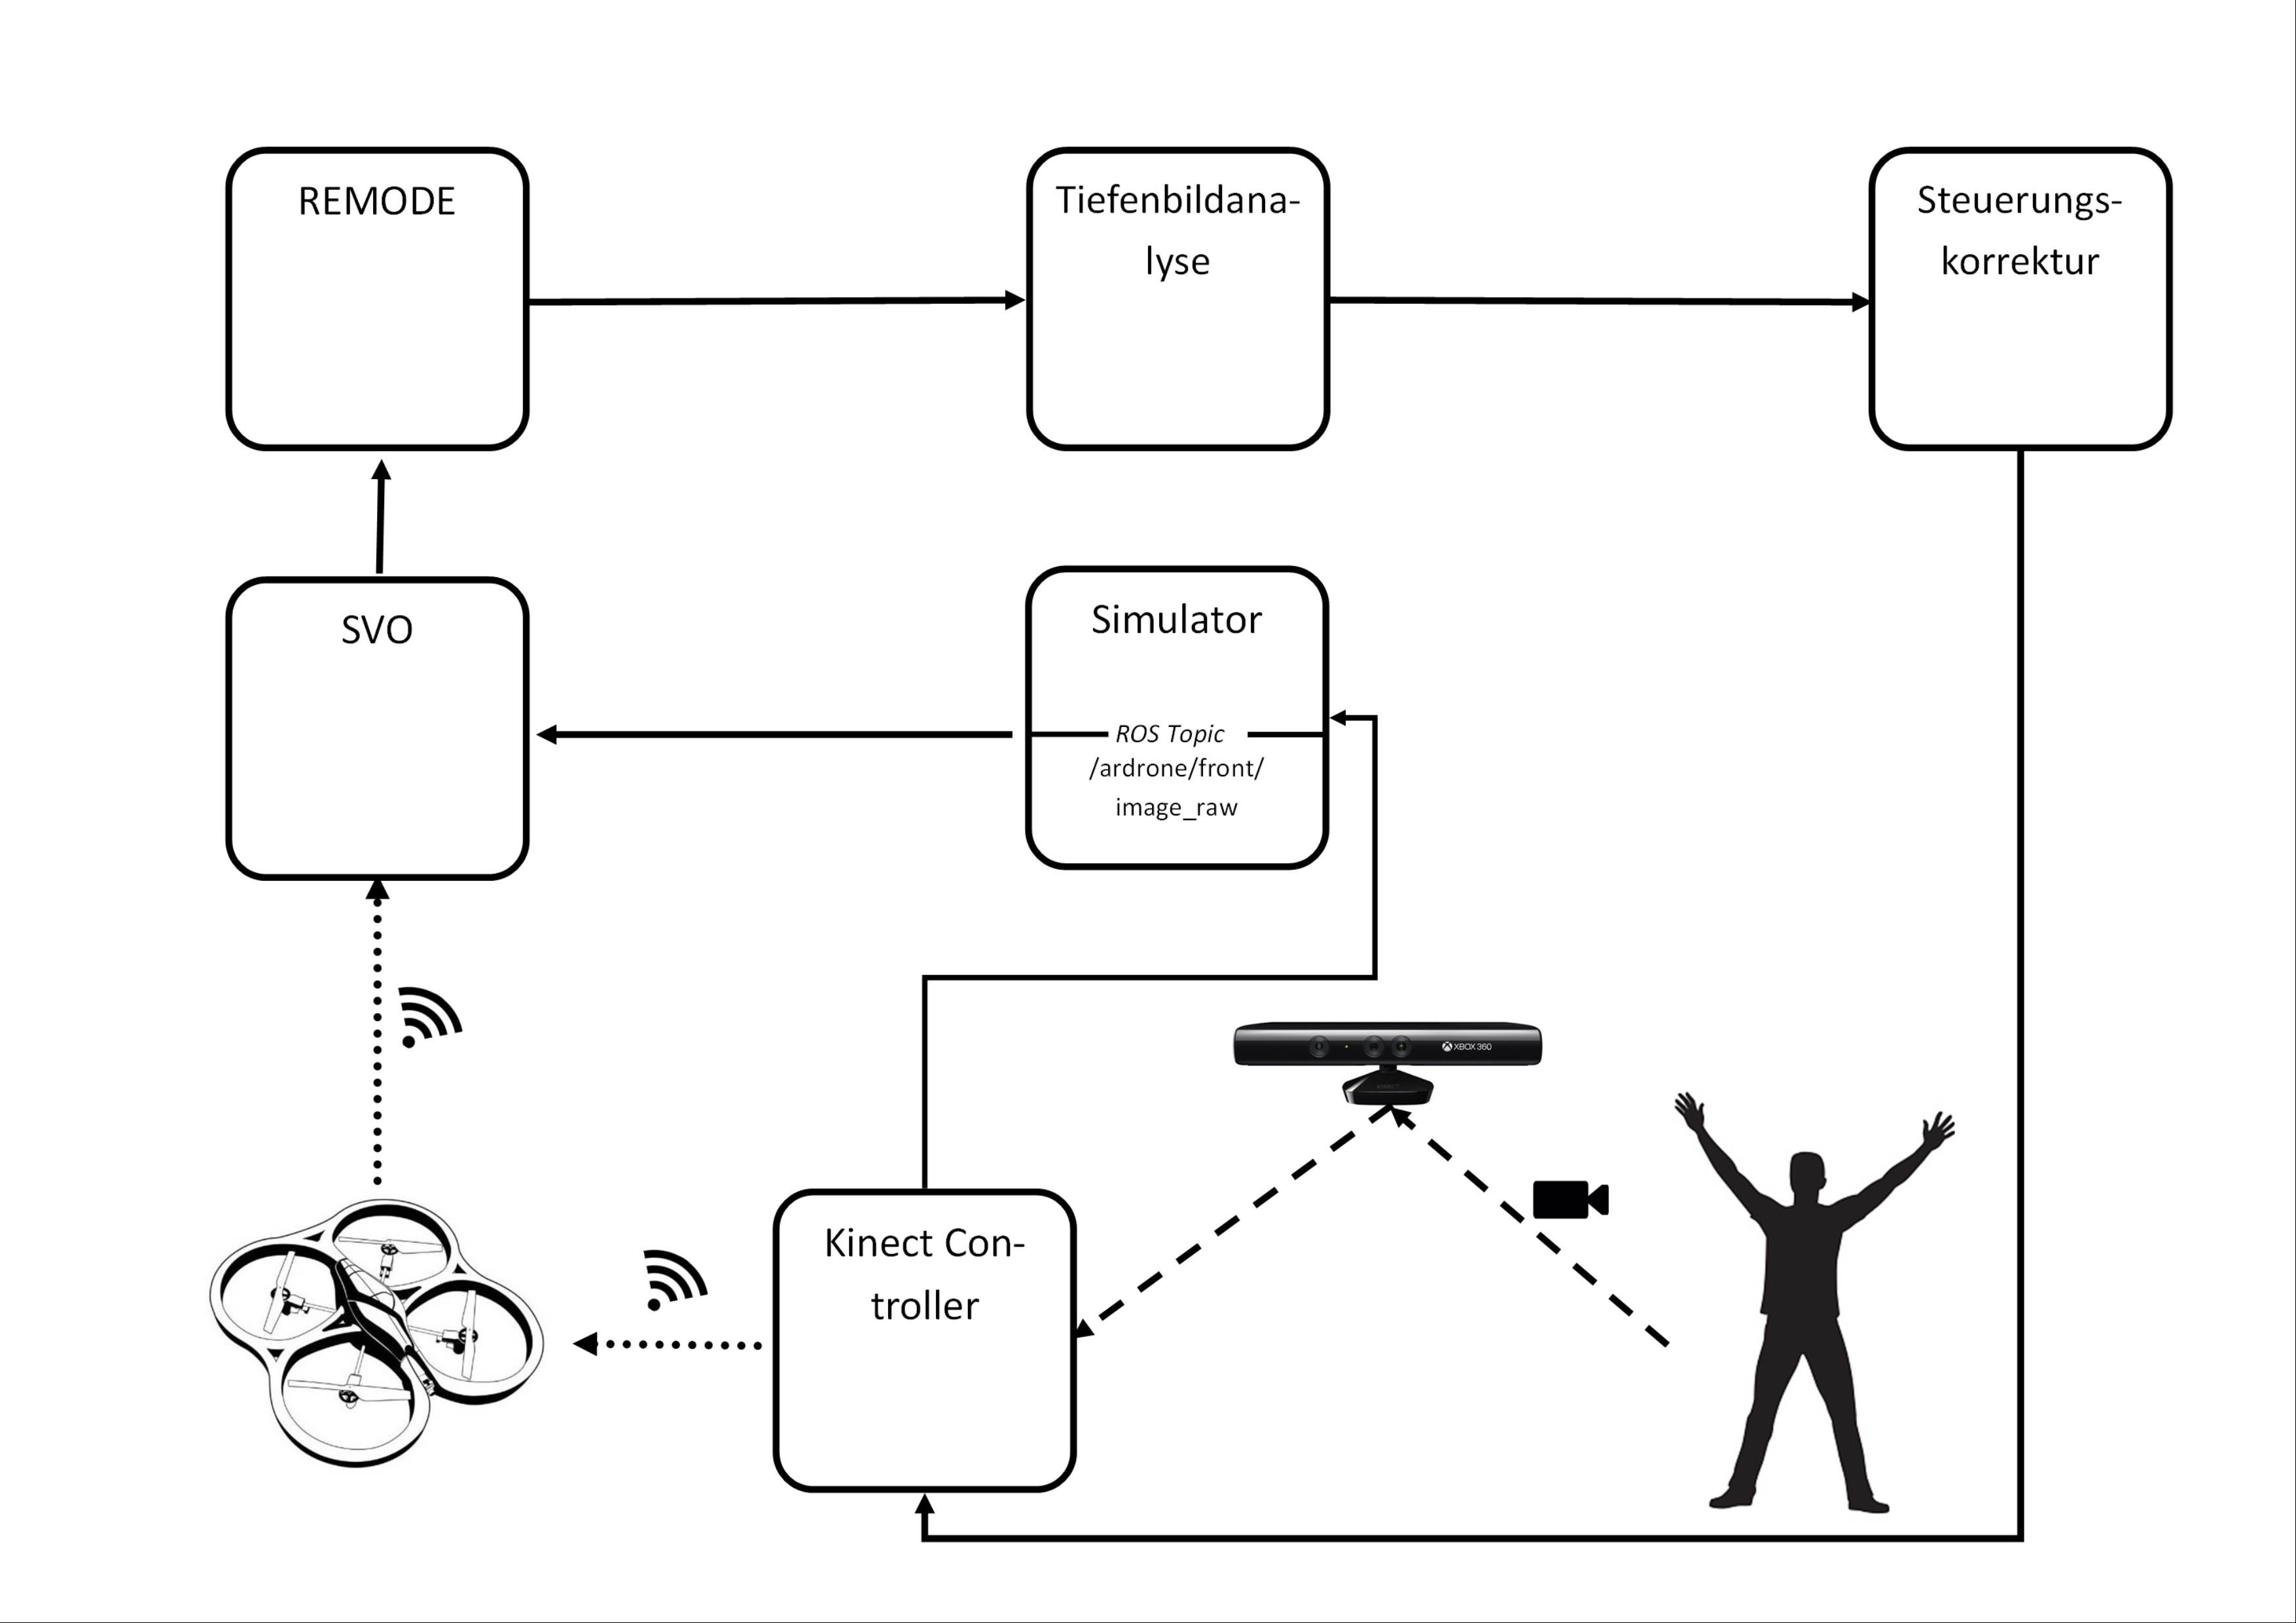
\includegraphics[scale=0.5, trim=4 4 4 4,clip]{Bilder/page01.jpg}
	\label{fig:architecture}
	\caption{Übersicht zur Softwarearchitektur}
\end{figure}
\newpage
\subsection{Ansteuerung der Kinect}
Der visuelle Sensor Microsoft Kinect dient als Nutzerschnittstelle zur Bedienung, indem der Nutzer Gesten benutzt um die Drohne zu steuern. Um die Sensoreingaben richtig verwenden zu können sind drei Schritte notwendig:
\begin{itemize}
	\item Korrekte Ansteuerung der Sensorhardware
	\item Körpererkennung und Tracking
	\item Verarbeitung der separaten Merkmale
\end{itemize}
Hierfür ist der erste Schritt die Hardware des Sensors richtig anzusteuern. Da die Microsoft Software nicht für Linux Systeme kompatibel ist, kommt einen Open Source Treiber zum Einsatz. Hierbei handelt es sich um OpenNI\cite{openni}, welches auch eine Middleware bereit stellt, um Körperbewegung und Gesten zur erkennen, beziehungsweise zu tracken. Die ROS-Node \grqq openni\_launch\grqq\cite{opennilaunch} realisiert die Ansteuerung des Kinect Sensors. Ebenfalls wird der zweite Schritt  Körpererkennung und Tracking  durch OpenNI gelöst, da die Middelware auch wie oben erwähnt dazu ist in der Lage ist. Die ROS-Node \grqq openni\_tracker\grqq\cite{opennitracker} ist dafür verantwortlich. Für den dritten Punkt Verarbeitung der seperaten Merkmale ist die selbst implementierte ROS-Node \grqq kinect\_controller\grqq \space zuständig. Dort werden die durch OpenNI extrahierten Merkmale, wie zum Beispiel linke Hand, rechte Hand, Kopf, usw. als Grundlage eingegeben. Ziel ist es die entsprechenden Befehle anhand der Eingaben für den Quadrocopter zu erstellen.
\begin{figure}[ht]
	\centering
	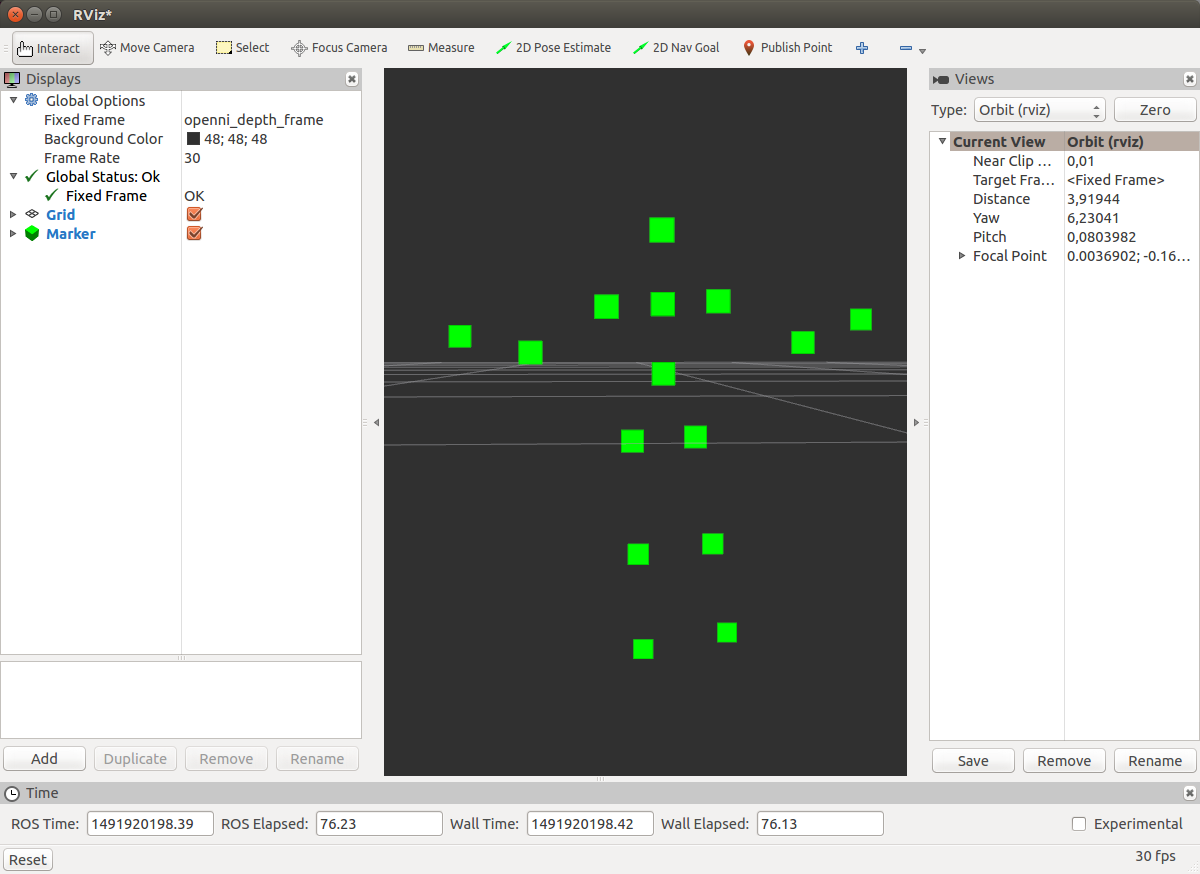
\includegraphics[scale=0.3]{Bilder/skeletonmarkers.png}
	\label{Darstellung der Körperteile in RVIZ}
	\caption{Darstellung der Körperteile in RVIZ}
\end{figure}
%Max
\newpage
\subsection{Kinect Controller}
Der Kinect Controller ist eine eigenständige ROS-Node, welche sich vorrangig um die Vorverarbeitung der Daten von der Kinect, in dem Falle die Ausgabe der Node des OpenNi Trackers, kümmert. Der Tracker veröffentlicht dauerhaft die aktuellen Transformationen, sowie Translationen der Koordinatensysteme der einzelnen Körperpunkte. Dies geschieht über die Topic \grqq /tf\grqq , wo die Nachrichten mit dem Typ \grqq TFMessage.msg\grqq \cite{tfmessage} \space verschickt werden. Die Klasse registriert sich bei der Initialisierung auf diesen Nachrichtenkanal und empfängt mithilfe der Methode \grqq messageCallback\grqq \space die Nachrichten. Allerdings wird pro erkanntem Merkmal jeweils eine Nachricht versandt, weswegen die berechneten Punkte mithilfe einer weiteren C++ Klasse \grqq SkeletonPoints\grqq \space aggregiert werden. Diese Klasse ist allein dafür ausgelegt um die einzelnen Punkte zu verwalten und somit für andere Komponenten einfach zugänglich zu machen. Die Zuordnung der Punkte geschieht mithilfe des Attributes \grqq child\_frame\_id\grqq der jeweiligen Nachricht in welchem der Name des erkannten Körperteils angegeben ist. Nachdem die Daten aggregiert wurden, kann mithilfe des Fuzzy Controllers berechnet werden, wie der Quadrocopter gesteuert werden soll. Dieser Steuerbefehl wird anschließend als Nachricht in der Topic \grqq /drone\_command\grqq \space publiziert. Dafür ist ein eigener Nachrichtentyp notwendig, welcher die Werte für die Geschwindigkeit für Pitch, Roll, Yaw, sowie für nach oben beziehungsweise unten.
\begin{figure}[ht]
	\centering
	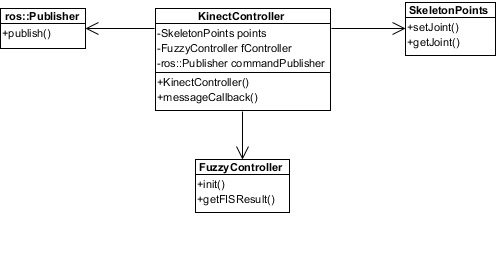
\includegraphics[scale=0.7]{Bilder/KinectController.jpg}
	\label{UML Klassendiagramm des Kinect Controllers}
	\caption{UML Klassendiagramm des Kinect Controllers}
\end{figure}
\subsection{Fuzzy Controller}
Der Fuzzy Controller ist in der C++ Klasse \grqq kinect\_controller\grqq \space integriert und somit kein eigenständige ROS-Node. Mithilfe der C++ Libary FuzzyLite\cite{fuzzylite} wird das erstellte Fuzzy Modell implementiert. Das in der Implementation verwendete Modell orientiert sich stark an dem Fuzzy Modell aus der Arbeit \grqq Gestensteuerung eines Flugroboters im AR-Kontext - I believe I can fly \grqq von Markus von Bergen et al. \cite{studienarbeitfly}, da der Sachverhalt ähnlich ist und nur lediglich kleine Anpassungen notwendig sind um es in der aktuellen Umgebung verwenden zu können. Es erhält die vier Eingabewerte aus den aggregierten Merkmalen und berechnet die korrespondierenden Geschwindigkeiten der vier möglichen Bewegungsrichtungen. Diese werden anschließend an die Node \grqq drone\_controller\grqq \space übergeben.
\subsection{Drone Controller}
Die ROS-Node \grqq drone\_controller\grqq \space ist der zentrale Punkt um den Quadrocopter anzusprechen. Die Notwendigkeit die Steuerung nochmals zu kapseln besteht aus dem Grund, dass mit der regulären Steuerung zwar Kommandos von verschiedenen Stellen gesendet werden können, aber eine nichtdeterministische Reihenfolge entsteht, da die Befehle in keinster Weise reguliert werden. Der Drone Controller übernimmt diese Aufgabe, indem er die Steuerung auf einer Ebene höher abstrahiert. Er kann Steuerbefehle über die Topic \grqq /drone\_command\grqq \space von mehreren Nodes gleichzeitig empfangen und diese Nachrichten anhand eines Indexes der Priorität unterschiedlich priorisieren. Dadurch ist es zum Beispiel für das Assistenzsystem möglich die Steuerbefehle des Nutzers zu korrigieren. Weiterhin können Befehle wie Landen, Starten oder der Notfallmodus ungehindert ausgeführt werden und ungewolltes Verhalten wird vermieden. Ebenfalls ist es möglich, dass zum Beispiel ein Spotter in den Flug eingreifen kann, wenn es zu Komplikationen kommt. Dadurch wird die Sicherheit des Fluggerätes und auch des Piloten verbessert. Theoretisch ist ebenso möglich durch geschicktes Priorisieren der Befehle mehr als ein Assistenzsystem gleichzeitig zu verwenden. Jedoch wird es mit zunehmender Anzahl schwieriger die richtigen Befehle auszuwählen und man sollte beachten, dass die Systeme sich nicht gegenseitig versuchen auszuhebeln. 
\subsection{ROS Nodes}
Für den gesamten Prozess von Nutzereingabe, durch den Kinectsensor, bis zur Steuerung der Drohne werden eine Vielzahl von Komponenten benötigt, da einige Arbeitsschritte notwendig sind, um die Daten zu verarbeiten. Zunächst wird die Microsoft Kinect durch die ROS-Node \grqq openni\_launch\grqq angesteuert und die Bilder der verschiedenen Kameras eingelesen. Anschließend werden diese Bilddaten durch die Node \grqq openni\_tracker \grqq analysiert und es wird, sofern ein Nutzer erkannt wurde ein Motion-Tracking erstellt. Dadurch werden bestimmte Features, in diesem Fall konkrete Körperteile erkannt. Diese werden als Nachricht unter der Topic \grqq/tf\grqq \space publiziert. Der kinect\_controller ist auf die Topic registriert und empfängt die gesendeten Nachrichten. Anhand der Merkmalspunkte werden vier Werte berechnet, die als Eingabe an die Fuzzy Logik übergeben werden. Anhand des Fuzzy Controllers ergeben sich vier Ausgangswerte, welche die Geschwindigkeiten für den Quadrocopter in den entsprechenden Richtungen, Neigung nach vorne beziehungsweise hinten, Neigung links und rechts, Rotation, sowie steigen und sinken angibt. Diese Befehle werden an die Node 
\grqq drone\_controller\grqq übergeben wo sie weiterverarbeitet werden. Ab dieser kann auch das Assistenzsystem eingreifen, indem es Korrektureingaben an den Controller sendet und die Steuerbefehle des Nutzer anpasst oder gar verwirft. Schließlich wird der Befehl an den Treiber in der Node \grqq ardrone\_autonomy\grqq \space übergeben, auf Hardwareebene übersetzt und an den Quadrocopter gesendet. Für den Fall, dass die Drohne nur simuliert wird, sendet wird der Befehl des \grqq drone\_controller\grqq direkt an die Simulationsumgebung und somit an den virtuellen Treiber gesendet. In der untenstehenden Abbildung wird die Kooperation der unterschiedlichen Nodes visualisiert. 
\begin{figure}[ht]
	\centering
	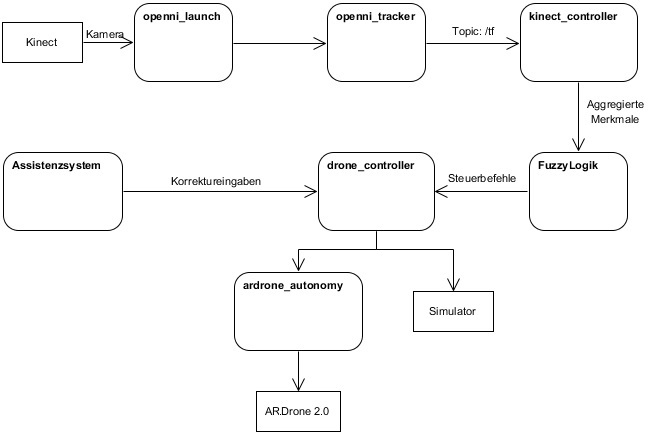
\includegraphics[scale=0.7]{Bilder/ros_nodes_flow.jpg}
	\label{Zusammenspiel der verschiedenen ROS-Nodes}
	\caption{Zusammenspiel der verschiedenen ROS-Nodes}
\end{figure}
%Beide
\newpage


%Bild der Drohne http://lightspots.ch/images/ARdronebw.png
%Bild vom Typ https://img.clipartfox.com/d02b01c31b79dd51b6c2c6a2a5db5985_stop-help-vector-art-outstretched-arm-clipart_416-416.jpeg
%Bild von kinect https://d3nevzfk7ii3be.cloudfront.net/igi/DtuTZhDHRWaOirBm.large


\newpage
\section{Assistenzsystem}
Im Kapitel \ref{Bildverarbeitung} wurde der Prozess beschrieben, wie aus den monokularen Aufnahmen der Frontkamera Tiefenbilder ermittelt werden können. Aufbauend darauf soll nun erarbeitet werden, wie mit Hilfe dieser Informationen die Implementation eines grundlegenden Assistenzsystems aussehen könnte.

\subsection{Problemanalyse}
%Christoph
Wie zuvor beschrieben, ist ein einfacher Anwendungsfall das Fliegen durch Hindernisse wie offene Türen. Dabei stößt man in der Bildverarbeitung auf eine Reihe von Herausforderungen. Wie in \ref{performanceprobleme} beschrieben, sind SVO und REMODE nicht optimal für den Anwendungsfall dieser Arbeit. Dabei treten Probleme vor allem bei der Analyse des Tiefenbildes auf. Dabei ist sowohl die niedrige Qualität der Tiefenbilder problematisch, als auch die hohe Zeit, welche zwischen den Bewegungen der Drohne und den Berechnungen der Tiefenpunktwolke vergehen kann. \newline
Die folgende Darstellung zeigt ein Beispiel für ein von REMODE berechnetes Bild.

\begin{figure}[ht]
	\centering
	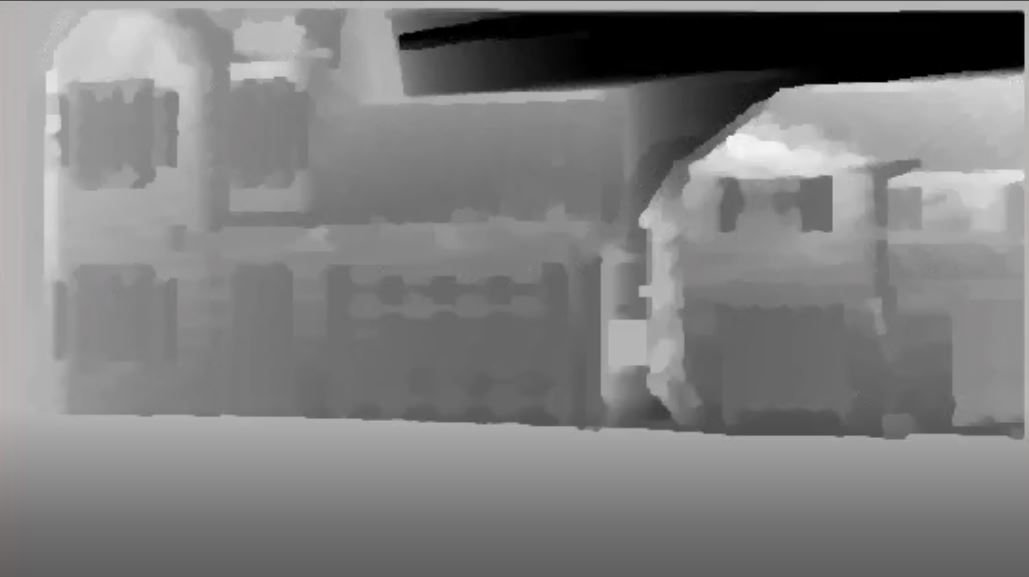
\includegraphics[scale=0.5]{Bilder/REMODE.jpg}
	\label{fig:REMODE}
	\caption{Approximiertes Tiefenbild durch REMODE}
\end{figure}

Dabei wird ersichtlich, das der grundlegende Kontext für einen menschlichen Betrachter verständlich ist - in diesem Fall sind dies zwei Häuser mit einer schmalen Lücke als Zwischenraum. Dabei sind genaue Texturen stark reduziert und teilweise verloren gegangen. Weiterhin sind Objektränder zum Teil von einem leichten hellen Schimmer umgeben, welcher in der Bildanalyse zu Problemen führen kann.


\subsection{Lösungsansätze}
Um mit solche einem Tiefenbild ein Objekt wie eine Tür, bzw. den Zwischenraum zu erkennen, gibt es verschiedene Ansätze, um die Punktwolke zu analysieren.

\subsubsection{Referenzobjekt}
Eine Möglichkeit ist die gezielte Suche nach definierten Abmessungen, Abständen und Formen im Bild. Dabei wird das Zielobjekt in die einzelnen Teilabschnitte aufgeteilt und die relative Beziehung dieser Teilstücke beschrieben. Am Beispiel einer Tür entspricht dies dem Rahmen, welcher aus zwei, zueinander parallelen, Geraden besteht, die rechtwinklig auf dem Untergrund aufliegen. Die beiden Geraden werden am Ende durch eine rechtwinklige Gerade miteinander verbunden. \newline

\begin{figure}[ht]
	\centering
	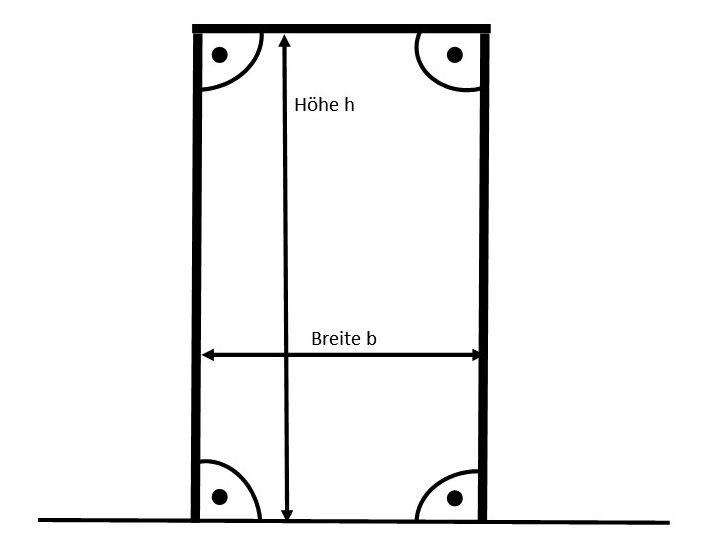
\includegraphics[scale=0.55]{Bilder/door.jpg}
	\label{fig:door}
	\caption{Objektreferenz einer Tür}
\end{figure}

Die Abbildung \ref{fig:door} visualisiert die beschriebenen Anforderungen. \newline
Wie in der vorherigen Darstellung \ref{fig:REMODE} erkennbar, gibt es keine klaren Kanten und Abgrenzungen. Dies erschwert einen Vergleich mit dem Referenzobjekt zusätzlich. Abhilfe für dieses Problem schaffen in der Bildverarbeitung Filter. Filtern ist eine Technik um Bilddaten zu modifizieren, oder sie in einer Art zu verbessern. Hauptsächlich wird diese Methode dafür genutzt, um hohe Frequenzen in einem Bild zu verringern, das Bild zu glätten, oder um niedrige Frequenzen zu verstärken, also um Kanten hervorzuheben. \newline
Filter basieren auf einer Berechnung in der Nachbarschaft\footnote{Die Nachbarschaft um einen Pixel ist eine Menge an Pixeln, die sich durch ihre relative Distanz zu diesem auszeichnen. \cite{filter1}} von Pixeln, wobei der Wert eines gegebenen Pixels im Ausgabebild bestimmt wird, in dem Algorithmen auf Pixel in der direkten Nachbarschaft dieses Datenpunktes angewandt werden. \cite{filter1}   \newline
Da die Tiefenbilder verwaschen und unscharf sind, müssen niedrige Frequenzen verstärkt werden. Ein Standard, um Kanten in einem Bild hervorzuheben ist der Marr-Hildreth-Operator oder auch Laplacian of Gaussian \textit{LoG} genannt. \cite{LoG} Dieser Algorithmus führt auf den Matrizen der Punktwolken des Eingangsbildes Faltungsoperationen \footnote{todo; was ist faltungsoperation} durch, um ein Ausgabebild mit verdeutlichten Kanten zu erzeugen. \newline
Dabei sucht der LoG nicht nach Kanten, sondern nach Gebieten mit rapiden Änderungen von Pixelintensitäten. Die zweite Ableitung erzeugt eine Kurve, bei der die beiden Seiten einer Kante durch einen positiven und einen negativen Wert gekennzeichnet sind. Die eigentliche Kante liegt hierbei an dem Punkt, wo der Graph Null durchquert. Die Abbildung \ref{fig:LoG} verdeutlicht dieses Verhalten.
\begin{figure}[ht]
	\centering
	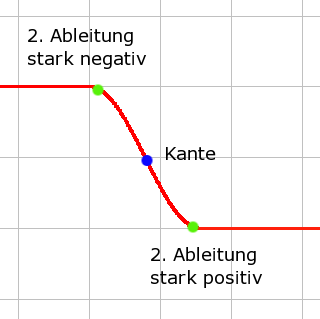
\includegraphics[scale=0.5]{Bilder/LoG.png}
	\label{fig:LoG}
	\caption{Verlauf der zweiten Ableitung im LoG Algorithmus \cite{LoG}}
\end{figure}
Die Point Cloud Library bietet dafür mit der Methode
\begin{center}
	\textit{pcl::Edge< PointInT, PointOutT >::detectEdgeLoG}
\end{center} 
eine Implementierung für diesen Algorithmus an. \cite{pclDocs} \newline
Nach dieser erste Schritt abgeschlossen ist, liegt ein Tiefenbild mit hervorgehobenen Kanten vor. Dies ist jedoch nicht ausreichend, um nun zuverlässig mit Hilfe eines Vergleichs mit dem Referenzobjekts z.B. Türen im Bild zu finden. \newline
Einerseits ist das Referenzobjekt grundsätzlich ein einfaches Rechteck. Diese gibt es potentiell sehr oft im Bild, wie beispielsweise Tische, Fenster oder Bilder an Wänden. Eine geöffnete Tür zeichnet sich dabei dadurch aus, dass der Inhalt des Rahmens weiter weg ist, also in der Punktwolke tiefer ist. Im Falle von sehr genauen Tiefenbildinformationen kann man an dieser Stelle mit einer hohen Wahrscheinlichkeit durch die Veränderung der Tiefe gute Ergebnisse bei der Suche erzielen. \newline
Wie bereits beschrieben ist das Tiefenbild jedoch sehr ungenau, da es nur durch einzelne Bilder approximiert wird. Somit ist die Verwendung eines Referenzobjektes und die Anwendung von Filtern zur Erkennung keine valide, praktisch einsetzbare Lösung. \newline

\subsubsection{Referenzpunktwolke}
Der zweite Ansatz basiert auf der Verwendung einer Referenzpunktwolke. Es wird somit kein relatives Objekt definiert, sondern man vergleicht die Punktwolke des gesamten Tiefenbildes, mit einer Punktwolke für eine Tür. \newline
Damit könnte ein besseres Ergebnis erzielt werden, da auch die Änderung der Tiefe zwischen Türrahmen und dem Bereich innerhalb des Rahmens betrachtet wird. Die Point Cloud Library bietet dafür eine Implementation an, welche als \textit{Correspondence Grouping}, also die Gruppierung nach Übereinstimmungen bezeichnet wird.

\begin{figure}[ht]
	\centering
	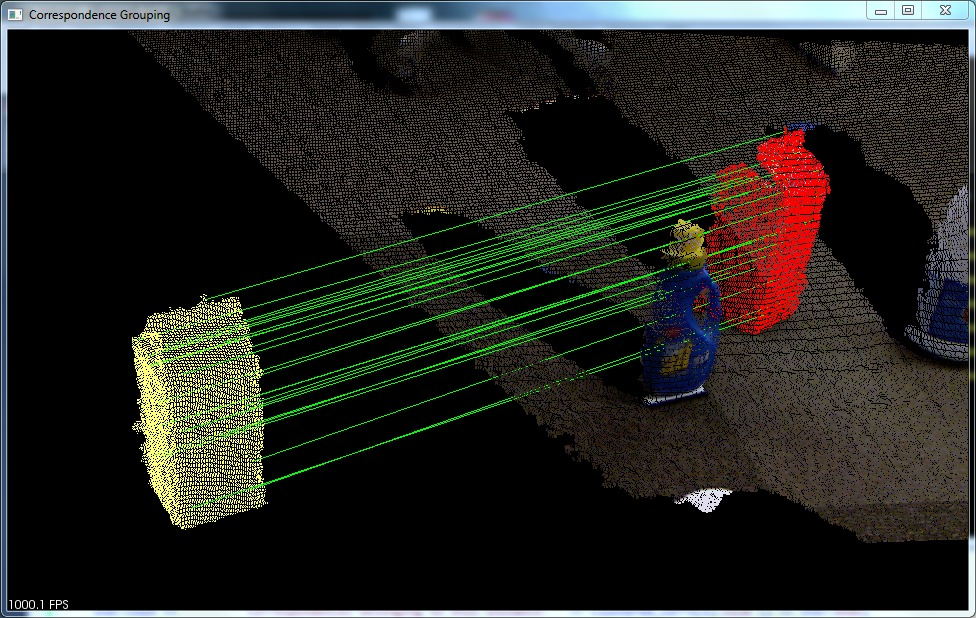
\includegraphics[scale=0.5]{Bilder/pcl_grouping.jpg}
	\label{fig:pcl_grouping}
	\caption{Correspondence Grouping mit dem PCL Algorithmus  \cite{pclGrouping}}
\end{figure}

Wie im Bild erkennbar wird mit Hilfe des Algorithmus versucht, Übereinstimmungen zwischen den Features der beiden Punktwolken zu finden. \newline
Schwierig ist hierbei die Auswahl und Generierung der Referenzpunktwolke. Es ist nicht möglich eine Lösung zu finden, die sowohl in der Simulation, als auch mit der realen Drohne funktioniert. Die Referenz ist immer nur dann sinnvoll, wenn sie nahezu exakt die gleichen Tiefeninformationen aufweist, wie das zu vergleichende Bild. \newline
Somit funktioniert die Auswertung auch nicht mehr, wenn eine leicht abgeänderte Tür verwendet wird, obwohl sich sowohl das Referenzobjekt, als auch das tatsächliche Objekt in der Simulation bzw. in der Realität befinden.
Weiterhin lassen sich die Tiefeninformationen eines bestimmten Objekts nur sehr schwer aus dem Gesamtbild extrahieren. Um dies zu erreichen müsste bereits bekannt sein, wo sich das Objekt im Bild befindet.
\subsubsection{Alternative Lösungen}
Weitere Überlegungen zur Objekterkennung sind spezielle Kennzeichnungen, die künstlich hinzugefügt werden. Denkbar sind beispielsweise farbliche Markierungen, wie ein roter Türrahmen, welcher sich farblich von der Umgebung abgrenzt und somit leicht zu finden ist. Dieser Ansatz ist grundsätzlich möglich und einfach umzusetzen, jedoch hat das Tiefenbild keine Farbinformationen. \newline
Es ist denkbar für dieses Zweck das Ausgangsbild zu verwenden, welches noch alle Farbinformationen besitzt, jedoch zweidimensional ist. Dies würde die Anforderungen an die Arbeit verletzen, da die Analyse nicht mehr auf den Tiefeninformationen basiert. \newline
Auch bei der Betrachtung anderer Objekte wie Wände kommt es zu schwerwiegenden Problemen. So kann der Abstand zwischen der Drohne und einer Wand in der Umgebung nicht genau genug bestimmt werden, um eine Kollision zu vermeiden, ohne unnötig in der Steuerung einzugreifen.